\section{Racionalna števila}

\begin{frame}
    \sectionpage

\end{frame}

\begin{frame}
    \tableofcontents[currentsection, hideothersubsections]
\end{frame}

%%% Ulomki in racionalna števila

    \subsection{Ulomki in racionalna števila}

        \begin{frame}
            \frametitle{Ulomki}

            \only<2->{\begin{alertblock}{}
                \textbf{Ulomek} $\frac{x}{y}$ je zapis, ki predstavlja zapis deljenja 
                \only<3->{$$x:y=\frac{x}{y};\quad y\neq 0\land x,y\in\mathbb{Z}.$$}
                \only<4->{Število/izraz $x$ imenujemo \textbf{števec}, $y$ pa \textbf{imenovalec}, med njima je \textbf{ulomkova črta}.}
            \end{alertblock}}

            \only<5->{\begin{block}{}
                Ulomek $\frac{x}{0}$ ni definiran (nima pomena), saj z $0$ ne moremo deliti.
            \end{block}}

            \only<6->{\begin{alertblock}{}
                \textbf{Algebrski ulomek} je ulomek, v katerem v števcu in/ali imenovalcu nastopajo algebrski izrazi.
            \end{alertblock}}

        \end{frame}

        \begin{frame}

            \only<2->{\begin{block}{}
                Vsako celo število $x\in\mathbb{Z}$ lahko zapišemo z ulomkom: $x=\frac{x}{1}$.
            \end{block}}

            \only<3->{\begin{block}{}
                \textbf{Ničelni ulomek} je ulomek oblike $\frac{0}{y}=0; y\neq 0$.
            \end{block}}

            \only<4->{\begin{block}{}
                V ulomku, kjer v števcu ali imenovalcu nastopa negativno število, upoštevamo enakost 
                \only<5->{$$-\frac{x}{y}=\frac{-x}{y}=\frac{x}{-y}.$$}
            \end{block}}

            \only<6->{\begin{alertblock}{}
                Vsakemu neničelnemu ulomku $\frac{x}{y}$ lahko priredimo njegovo \textbf{obratno vrednost}: 
                \only<7->{$$\left(\frac{x}{y}\right)^{-1}=\frac{y}{x}; \quad x,y\in\mathbb{Z}\setminus\{0\}.$$}
            \end{alertblock}}

        \end{frame}


        \begin{frame}
            \frametitle{Racionalna števila}

            \only<2->{\begin{block}{}
                Množica racionalnih števil $\mathbb{Q}$ je sestavljena iz vseh ulomkov (kar pomeni, da vsebuje tudi vsa naravna in cela števila).
            \end{block}}

            \only<3->{\begin{block}{}
                \centering
                \begin{tikzpicture}
                    % \clip (0,0) rectangle (14.000000,10.000000);
                    {\footnotesize
                    
                    % Drawing segment A B
                    \draw [line width=0.016cm] (1.000000,1.500000) -- (4.460000,1.500000);%
                    \draw [line width=0.016cm] (4.540000,1.500000) -- (8.000000,1.500000);%
                    
                    % Marking point 0 by circle
                    \draw [line width=0.016cm] (4.500000,1.500000) circle (0.040000);%
                    \draw (4.500000,1.500000) node [anchor=south] { $0$ };%
                    
                    \only<7->{
                    % Changing color 255 0 0
                    \definecolor{r255g0b0}{rgb}{1.000000,0.000000,0.000000}%
                    \color{r255g0b0}% 
                    
                    % Marking point \mathbb{Q}^+
                    \draw (6.250000,1.500000) node [anchor=south] { $\mathbb{Q}^+$ };%
                    
                    % Drawing segment B 0
                    \draw [line width=0.016cm] (8.000000,1.500000) -- (4.540000,1.500000);%
                    }

                    \only<5->{
                    % Changing color 0 255 0
                    \definecolor{r0g255b0}{rgb}{0.000000,1.000000,0.000000}%
                    \color{r0g255b0}% 
                    
                    % Marking point \mathbb{Q}^-
                    \draw (2.750000,1.500000) node [anchor=south] { $\mathbb{Q}^-$ };%
                    
                    % Drawing segment A 0
                    \draw [line width=0.016cm] (1.000000,1.500000) -- (4.460000,1.500000);%
                    }

                    % Changing color 0 0 0
                    \definecolor{r0g0b0}{rgb}{0.000000,0.000000,0.000000}%
                    \color{r0g0b0}% 
                    
                    % Marking point \mathbb{Q}
                    \draw (1.500000,2.000000) node  { $\mathbb{Q}$ };%
                    \color{black}
                    }
                    \end{tikzpicture}
                    
            \end{block}}

            \only<4->{\begin{block}{}
                Glede na predznak razdelimo racionalna števila v tri množice:
                \begin{itemize}
                    \item<5-> \textcolor{green}{množico negativnih racionalnih števil $\mathbf{\mathbb{Q}^-}$},
                    \item<6-> množico z elementom nič: $\mathbf{\{0\}}$ in
                    \item<7-> \textcolor{red}{množico pozitivnih racionalnih števil: $\mathbf{\mathbb{Q}^+}$}.
                \end{itemize}
                $$ \mathbb{Q}=\only<4->{\textcolor{green}{\mathbb{Q}^-}}\only<5->{\cup\{0\}}\only<6->{\cup\textcolor{red}{\mathbb{Q}^+}} $$
            \end{block}}
            

            % \only<7->{\begin{block}{}
            %     Množica racionalnih števil je povsod gosta, saj lahko med poljubnima racionalnima številoma vedno najdemo racionalno število (posledično je med dvema racionalnima številoma neskončno mnogo racionalnih števil).
            % \end{block}}

        \end{frame}

        \begin{frame}
            \only<2->{\begin{block}{}
                Ulomka $\frac{x}{y}$ in $\frac{z}{w}$ sta enaka/enakovredna natanko takrat, ko je $xz=wy$; $y,z\neq 0$.
                \only<3->{$$\frac{x}{y}=\frac{w}{z}\Leftrightarrow xz=wy; \quad y,z\neq 0$$}
            \end{block}}

            \only<4->{\begin{block}{}
                Enaka/enakovredna ulomka sta različna zapisa za isto racionalno število.
            \end{block}}
        \end{frame}



%%% naloge

        \begin{frame}
            \only<2->{\begin{exampleblock}{Naloga}
                Za katere vrednosti $x$ ulomek ni definiran?
                \only<3->{\begin{itemize}
                    \item $\dfrac{x-2}{x+1}$ \\~\\~
                    \item $\dfrac{2}{x-5}$ \\~\\~
                    \item $\dfrac{x+2}{3}$ \\~\\~
                    \item $\dfrac{13}{2x-5}$ \\~\\~
                \end{itemize}}
            \end{exampleblock}}
        \end{frame}

        \begin{frame}
            \only<2->{\begin{exampleblock}{Naloga}
                Za katere vrednosti $x$ ima ulomek vrednost enako $0$?
                \only<3->{\begin{itemize}
                    \item $\dfrac{x-2}{x+1}$ \\~\\~
                    \item $\dfrac{2}{x-5}$ \\~\\~
                    \item $\dfrac{x+2}{3}$ \\~\\~
                    \item $\dfrac{13}{2x-5}$ \\~\\~
                \end{itemize}}
            \end{exampleblock}}
        \end{frame}

        \begin{frame}
            \only<2->{\begin{exampleblock}{Naloga}
                Ali imata ulomka isto vrednost?
                \only<3->{\begin{itemize}
                    \item $\dfrac{2}{3}$ in $\dfrac{10}{15}$ \\~\\~
                    \item $\dfrac{-1}{2}$ in $\dfrac{1}{-2}$ \\~\\~
                    \item $\dfrac{4}{5}$ in $\dfrac{-8}{-10}$ \\~\\~
                    \item $\dfrac{5}{8}$ in $\dfrac{8}{5}$ \\~\\~
                \end{itemize}}
            \end{exampleblock}}
        \end{frame}

        \begin{frame}
            \only<2->{\begin{exampleblock}{Naloga}
                Za kateri $x$ imata ulomka isto vrednost?
                \only<3->{\begin{itemize}
                    \item $\dfrac{x+1}{2}$ in $\dfrac{3}{4}$ \\~\\~
                    \item $\dfrac{4}{2x-1}$ in $\dfrac{1}{3}$ \\~\\~
                    \item $\dfrac{x+1}{2}$ in $\dfrac{x-1}{-3}$ \\~\\~
                    \item $\dfrac{x+1}{x-2}$ in $\dfrac{2}{5}$ \\~\\~
                \end{itemize}}
            \end{exampleblock}}
        \end{frame}

        \begin{frame}
            \only<2->{\begin{exampleblock}{Naloga}
                Ali ulomka predstavljata isto vrednost?
                \only<3->{\begin{itemize}
                    \item $\left(\dfrac{1}{2}\right)^{-1}$ in $-\dfrac{1}{2}$ \\~\\~
                    \item $\left(\dfrac{2}{3}\right)^{-1}$ in $\dfrac{3}{2}$ \\~\\~
                    \item $ 1\dfrac{3}{7}$ in $\left(\dfrac{7}{10}\right)^{-1}$ \\~\\~
               \end{itemize}}
            \end{exampleblock}}
        \end{frame}

        \begin{frame}
            \only<2->{\begin{exampleblock}{Naloga}
                Ali ulomka predstavljata isto vrednost?
                \only<3->{\begin{itemize}
                    \item $ 2\cdot\dfrac{3}{4}$ in $\dfrac{3}{2}$ \\~\\~
                    \item $ 2\dfrac{3}{4}$ in $\dfrac{3}{2}$ \\~\\~
                    \item $\left(1\dfrac{2}{5}\right)^{-1}$ in $ 1\dfrac{5}{2}$ \\~\\~
                    \item $\left(1\dfrac{2}{5}\right)^{-1}$ in $\dfrac{5}{7}$ \\~\\~
               \end{itemize}}
            \end{exampleblock}}
        \end{frame}

        \begin{frame}
            \only<2->{\begin{exampleblock}{Naloga}
                Zapišite s celim delom oziroma z ulomkom.
                \only<3->{\begin{itemize}
                    \begin{columns}
                        \column{0.4\textwidth}
                            \item $\dfrac{14}{5}$ \\~\\~
                            \item $-\dfrac{5}{2}$ \\~\\~
                            \item $\dfrac{4}{3}$ \\~\\~
    
                        \column{0.4\textwidth}
                            \item $\dfrac{110}{17}$ \\~\\~
                            \item $ 3\dfrac{5}{8}$ \\~\\~
                            \item $ 2\dfrac{9}{2}$ \\~\\~                 
                        \end{columns}

               \end{itemize}}
            \end{exampleblock}}
        \end{frame}

        % \begin{frame}
        %     \only<2->{\begin{exampleblock}{Naloga}
        %         Poenostavite.
        %         \only<3->{\begin{itemize}
        %             \item a \\~
        %         \end{itemize}}
        %     \end{exampleblock}}
        % \end{frame}

        % \begin{frame}
        %     \only<2->{\begin{exampleblock}{Naloga}
        %         Poenostavite.
        %         \only<3->{\begin{itemize}
        %             \item a \\~
        %         \end{itemize}}
        %     \end{exampleblock}}
        % \end{frame}

        %%% Razširjanje in krajšanje ulomkov

    \subsection{Razširjanje in krajšanje ulomkov}

        \begin{frame}
            \frametitle{Razširjanje in krajšanje ulomkov}

            \only<2->{\begin{alertblock}{Razširjanje ulomka}
                \only<3->{Ulomek ohrani svojo vrednost, če števec in imenovalec pomnožimo z istim neničelnim številom oziroma izrazom.
                Temu postopku pravimo \textbf{razširjanje ulomka}.}

                \only<4->{$$\dfrac{x}{y}=\dfrac{x\cdot z}{y\cdot z}; \quad x\in\mathbb{Z} \land y,z\in\mathbb{Z}\setminus\{0\}$$}
            \end{alertblock}}

            \only<5->{\begin{block}{}
                Ko ulomke seštevamo ali odštevamo, jih razširimo na \textbf{najmanjši skupni imenovalec}, 
                ki je najmanjši skupni večkratnik vseh imenovalcev.
            \end{block}}

        \end{frame}

        \begin{frame}
            \only<2->{\begin{alertblock}{Krajšanje ulomka}
                \only<3->{Vrednost ulomka se ne spremeni, če števec in imenovalec delimo z istim neničelnim številom oziroma izrazom.
                Temu postopku rečemo \textbf{krajšanje ulomka}.}

                \only<4->{$$\dfrac{x\cdot z}{y\cdot z}=\dfrac{x}{y}; \quad x\in\mathbb{Z}\land y,z\in\mathbb{Z}\setminus\{0\} $$}
            \end{alertblock}}

            \only<5->{\begin{alertblock}{Okrajšan ulomek}
                \only<6->{Ulomek $\dfrac{x}{y}$ je \textbf{okrajšan}, če je $(x,y)=1$, torej če sta števec in imenovalec tuji števili.}
            \end{alertblock}}
        \end{frame}


        %%% naloge

        \begin{frame}
            \only<2->{\begin{exampleblock}{Naloga}
                Razširite ulomke na najmanjši skupni imenovalec.
                \only<3->{\begin{itemize}
                    \begin{columns}
                        \column{0.4\textwidth}
                            \item $\dfrac{1}{3}$, $\dfrac{3}{5}$ in $\dfrac{5}{6}$ \\~\\~
                            \item $\dfrac{2}{7}$, $1$ in $\dfrac{1}{2}$ \\~\\~
                            \item $\dfrac{5}{6}$, $\dfrac{1}{2}$ in $-\dfrac{2}{3}$ \\~\\~

                        \column{0.4\textwidth}
                            \item $\dfrac{1}{5}$, $-\dfrac{1}{2}$ in $\dfrac{-1}{3}$ \\~\\~
                            \item $\dfrac{2}{-1}$, $\dfrac{3}{2}$ in $\dfrac{1}{-3}$ \\~\\~
                            \item $\dfrac{3}{-4}$, $\dfrac{-1}{2}$ in $-\dfrac{2}{5}$ \\~\\~

                    \end{columns}
                \end{itemize}}
            \end{exampleblock}}
        \end{frame}

        \begin{frame}
            \only<2->{\begin{exampleblock}{Naloga}
                Razširite ulomke na najmanjši skupni imenovalec.
                \only<3->{\begin{itemize}
                    \begin{columns}
                        \column{0.4\textwidth}
                            \item $\dfrac{1}{x-1}$, $\dfrac{1}{x+1}$ in $1$ \\~\\~
                            \item $\dfrac{2}{x}$, $\dfrac{1}{x-3}$ in $\dfrac{1}{(x-3)^2}$ \\~\\~
                            \item $\dfrac{3}{x^2-4x}$, $\dfrac{1}{x}$ in $\dfrac{2}{x-4}$ \\~

                        \column{0.4\textwidth}
                            \item $\dfrac{4}{x-4}$, $\dfrac{2}{x-2}$ in $\dfrac{1}{x^2-6x+8}$ \\~\\~
                            \item $\dfrac{2}{x-1}$ in $\dfrac{3}{1-x}$ \\~\\~
                            \item $\dfrac{1}{2-x}$, $\dfrac{2}{x+2}$ in $\dfrac{3}{x^2-4}$ \\~\\~

                    \end{columns}

                \end{itemize}}
            \end{exampleblock}}
        \end{frame}

        \begin{frame}
            \only<2->{\begin{exampleblock}{Naloga}
                Okrajšajte ulomek.
                \only<3->{\begin{itemize}
                    \item $\dfrac{100}{225}$ \\~\\~
                    \item $\dfrac{34}{51}$ \\~\\~
                    \item $\dfrac{121}{3}$ \\~\\~
                    \item $\dfrac{45}{75}$ \\~\\~
                \end{itemize}}
            \end{exampleblock}}
        \end{frame}

        \begin{frame}
            \only<2->{\begin{exampleblock}{Naloga}
                Okrajšajte ulomek.
                \only<3->{\begin{itemize}
                    \begin{columns}
                        \column{0.4\textwidth}
                            \item $\dfrac{x^2-4}{x^2+2x}$ \\~\\~
                            \item $\dfrac{x^3+8}{2x+4}$ \\~\\~
                            \item $\dfrac{x^3-1}{x^2-4x+3}$ \\~\\~

                        \column{0.4\textwidth}
                            \item $\dfrac{x^3-2x^2-x+2}{x^2-3x+2}$ \\~\\~
                            \item $\dfrac{x^2-9}{3-x}$ \\~\\~
                            \item $\dfrac{x-4}{16-x^2}$ \\~\\~

                    \end{columns}

                \end{itemize}}
            \end{exampleblock}}
        \end{frame}

        % \begin{frame}
        %     \only<2->{\begin{exampleblock}{Naloga}
        %         Poenostavite.
        %         \only<3->{\begin{itemize}
        %             \item a \\~
        %         \end{itemize}}
        %     \end{exampleblock}}
        % \end{frame}

        % \begin{frame}
        %     \only<2->{\begin{exampleblock}{Naloga}
        %         Poenostavite.
        %         \only<3->{\begin{itemize}
        %             \item a \\~
        %         \end{itemize}}
        %     \end{exampleblock}}
        % \end{frame}


%%% Seštevanje in odštevanje ulomkov

        \subsection{Seštevanje in odštevanje ulomkov}

        \begin{frame}
            \frametitle{Seštevanje in odštevanje ulomkov}

            \only<2->{\begin{alertblock}{Seštevanje ulomkov}
                \only<3->{Ulomke \textbf{seštevamo} tako, da jih razširimo na skupni imenovalec, nato seštejemo števce, imenovalce pa prepišemo.}
                \only<4->{$$\dfrac{x}{y}+\dfrac{z}{w}=\dfrac{xw}{yw}+\dfrac{yz}{yw}=\dfrac{xw+yz}{yw}; \quad x,z\in\mathbb{Z}\land y,w\in\mathbb{Z}\setminus\{0\} $$}
            \end{alertblock}}

            \only<5->{\begin{alertblock}{Odštevanje ulomkov}
                \only<6->{Ulomke \textbf{odštevamo} tako, da prištejemo nasprotni ulomek.}
                \only<7->{$$\dfrac{x}{y}-\dfrac{z}{w}=\dfrac{x}{y}+\left(-\dfrac{z}{w}\right)=\dfrac{xw}{yw}+\dfrac{-yz}{yw}=\dfrac{xw-yz}{yw}; \quad x,z\in\mathbb{Z}\land y,w\in\mathbb{Z}\setminus\{0\} $$}
            \end{alertblock}}

    
        \end{frame}


%%% naloge
        \begin{frame}
            \only<2->{\begin{exampleblock}{Naloga}
                Izračunajte.
                \only<3->{\begin{itemize}
                    \item $\dfrac{5}{7}+\dfrac{1}{14}$ \\~\\~
                    \item $\dfrac{2}{9}-\dfrac{1}{3}$ \\~\\~
                    \item $\dfrac{3}{8}+1\dfrac{1}{2}$ \\~\\~
                    \item $1-\dfrac{5}{6}$ \\~\\~
                \end{itemize}}
            \end{exampleblock}}
        \end{frame}

        \begin{frame}
            \only<2->{\begin{exampleblock}{Naloga}
                Izračunajte.
                \only<3->{\begin{itemize}
                    \item $\left(\dfrac{2}{3}-2\dfrac{1}{4}\right)+\dfrac{1}{12}$ \\~\\~
                    \item $\dfrac{2}{7}-\dfrac{3}{4}+\left(\dfrac{1}{2}-2\right)$ \\~\\~
                    \item $\left(\dfrac{2}{3}-\left(\dfrac{1}{3}-3\right)+\dfrac{1}{4}\right)-\dfrac{1}{2}$ \\~\\~
                    \item $1-\left(2-\left(3-4-\left(5-\dfrac{1}{2}\right)\right)+\dfrac{1}{3}\right)$ \\~\\~
                \end{itemize}}
            \end{exampleblock}}
        \end{frame}


        \begin{frame}
            \only<2->{\begin{exampleblock}{Naloga}
                Poenostavite.
                \only<3->{\begin{itemize}
                    \item $\dfrac{x}{x-1}-\dfrac{x}{x+1}$ \\~\\~
                    \item $\dfrac{3}{x^2}+\dfrac{4}{x^3}-\dfrac{1}{x}$ \\~\\~
                    \item $\dfrac{3}{x^2-4x}-\left(\dfrac{1}{x-4}+\dfrac{2}{x^2-5x+4}\right)$ \\~\\~
                    \item $\dfrac{2}{xy}+\dfrac{3}{x}-\dfrac{2}{y}$ \\~\\~
                \end{itemize}}
            \end{exampleblock}}
        \end{frame}


        \begin{frame}
            \only<2->{\begin{exampleblock}{Naloga}
                Poenostavite.
                \only<3->{\begin{itemize}
                    \item $\dfrac{(x-3)^2+(x+3)^2}{x^2-9}-\dfrac{3x^2}{2x^2-x^2}$ \\~\\~
                    \item $\dfrac{(a-3)^3-(a-1)^3+26}{6a}+\left(-\dfrac{1}{2}\right)^{-1}$ \\~\\~
                    \item $\dfrac{x^3-2x^2-x+2}{-x(1-x)-2}-\left(\dfrac{x-1}{x}-1\right)^{-1}$ \\~\\~
                    \item $\left(\dfrac{x}{2}-\left(\dfrac{x}{3}-\left(\dfrac{x}{4}-\dfrac{x}{5}\right)\right)\right)-\left(\dfrac{60}{x}\right)^{-1}$ \\~\\~
                \end{itemize}}
            \end{exampleblock}}
        \end{frame}


        %%% Množenje ulomkov
        
        \subsection{Množenje ulomkov}

        \begin{frame}
            \frametitle{Množenje ulomkov}

            \only<2->{\begin{alertblock}{Množenje ulomkov}
                \only<3->{Ulomka \textbf{množimo} tako, da števce množimo s števci, imenovalce pa množimo z imenovalci.}
                \only<4->{$$\dfrac{x}{y}\cdot \dfrac{z}{w}=\dfrac{xz}{yw}; \quad x,z\in\mathbb{Z}\land y,w\in\mathbb{Z}\setminus\{0\}$$}
                
            \end{alertblock}}

            \only<5->{\begin{block}{}
                Produkt danega in njemu obratnega ulomka je enak $1$.
                \only<6->{$$\dfrac{x}{y}\cdot\left(\dfrac{x}{y}\right)^{-1}=\dfrac{x}{y}\cdot\dfrac{y}{x}=1$$}
            \end{block}}
        \end{frame}

        %%% naloge

        \begin{frame}
            \only<2->{\begin{exampleblock}{Naloga}
                Izračunajte.
                \only<3->{\begin{itemize}
                    \begin{columns}
                        \column{0.4\textwidth}
                            \item $\dfrac{1}{3}\cdot \dfrac{3}{7}$ \\~\\~
                            \item $\dfrac{-2}{13}\cdot \left(-\dfrac{39}{4}\right)$ \\~\\~
                            \item $\dfrac{2}{5}\cdot \dfrac{4}{9}$ \\~\\~

                        \column{0.4\textwidth}
                            \item $2\dfrac{1}{3}\cdot 3\dfrac{3}{4}$ \\~\\~
                            \item $\dfrac{-2}{5}\cdot 4\dfrac{2}{7}$ \\~\\~
                            \item $3\cdot\dfrac{2}{3}$ \\~\\~

                    \end{columns}

                \end{itemize}}
            \end{exampleblock}}
        \end{frame}


        \begin{frame}
            \only<2->{\begin{exampleblock}{Naloga}
                Poenostavite.
                \only<3->{\begin{itemize}
                    \item $\dfrac{x^2-9}{x^2+3x+9}\cdot\dfrac{x^3-27}{x^2-6k+9}$ \\~\\~
                    \item $\dfrac{x^2+5x}{-x+2}\cdot\dfrac{2x^2-8}{x^2+7x+10}$ \\~\\~
                    \item $\dfrac{x^3-4x^2-4x+16}{2x+4}\cdot\dfrac{6x}{3x-6}$ \\~\\~
                    \item $2\cdot\dfrac{x}{x-1}\cdot\dfrac{x^2-1}{x^2+x}$ \\~\\~
                \end{itemize}}
            \end{exampleblock}}
        \end{frame}


        \begin{frame}
            \only<2->{\begin{exampleblock}{Naloga}
                Poenostavite.
                \only<3->{\begin{itemize}
                    \item $\dfrac{x^2-4}{x^2-1}\cdot\dfrac{x^3-1}{x^3+x^2+x}\cdot\dfrac{x^2+x}{2-x}$ \\~\\~
                    \item $\left(\dfrac{6-x}{x^2+6x}-\dfrac{x}{36-x^2}\right)\cdot\left(\dfrac{2x-6}{x^2+6x}\right)^{-1}+\dfrac{x}{6-x}$ \\~\\~
                    \item $\left(\left(x-y+\left(\dfrac{x+y}{2xy}\right)^{-1}\right)\cdot\left(\dfrac{1}{x+y}\right)^{-1}-2xy\right)\cdot(x-y)^{-1}$ \\~\\~
                    \item $\left(xy+y^2-\dfrac{xy+y^2}{3xy-3x^2}\right)\cdot\left(\dfrac{x+y}{3x}\right)^{-1}-\left(-\dfrac{y-x}{y}\right)^{-1}$ \\~\\~
                \end{itemize}}
            \end{exampleblock}}
        \end{frame}



        %%% Deljenje ulomkov

        \subsection{Deljenje ulomkov}

        \begin{frame}
            \frametitle{Deljenje ulomkov}

            \only<2->{\begin{alertblock}{Deljenje ulomkov}
                \only<3->{Ulomek \textbf{delimo} z neničelnim ulomkom tako, da prvi ulomek množimo z obratno vrednostjo drugega ulomka.}
                \only<4->{$$\dfrac{x}{y}:\dfrac{z}{w}=\dfrac{x}{y}\cdot\left(\dfrac{z}{w}\right)^{-1}=\dfrac{x}{y}\cdot\dfrac{w}{z}=\dfrac{xw}{yz}; \quad x\in\mathbb{Z}\land y,z,w\in\mathbb{Z}\setminus\{0\} $$}
            \end{alertblock}}

            \only<5->{\begin{alertblock}{}
                Deljenju ulomkov lahko zapišemo kot \textbf{dvojni ulomek}.
                \only<6->{$$\dfrac{x}{y}:\dfrac{z}{w}=\dfrac{\frac{x}{y}}{\frac{z}{w}}; \quad x\in\mathbb{Z}\land y,z,w\in\mathbb{Z}\setminus\{0\} $$}
            \end{alertblock}}

        \end{frame}


        %%% naloge

        \begin{frame}
            \only<2->{\begin{exampleblock}{Naloga}
                Izračunajte.
                \only<3->{\begin{itemize}
                    \item $2:\dfrac{4}{5}$ \\~\\~
                    \item $1\dfrac{2}{3}:2\dfrac{5}{6}$ \\~\\~
                    \item $\dfrac{7}{12}:14$ \\~\\~
                    \item $\dfrac{3}{8}:\dfrac{9}{32}$ \\~\\~
                \end{itemize}}
            \end{exampleblock}}
        \end{frame}


        \begin{frame}
            \only<2->{\begin{exampleblock}{Naloga}
                Izračunajte.
                \only<3->{\begin{itemize}
                    \begin{columns}
                        \column{0.4\textwidth}
                            \item $\dfrac{\dfrac{3}{4}}{\dfrac{6}{8}}$ \\~\\~
                            \item $\dfrac{\dfrac{1}{2}}{2}$ \\~\\~
                            \item $\dfrac{3}{\dfrac{5}{6}}$ \\~\\~
                        \column{0.4\textwidth}
                            \item $\dfrac{\dfrac{2}{-5}}{\dfrac{-1}{5}}$ \\~\\~
                            \item $\dfrac{\dfrac{3}{5}}{-2}$ \\~\\~
                            \item $\dfrac{-\dfrac{1}{2}}{2^{-1}}$ \\~\\~
                    \end{columns}

                \end{itemize}}
            \end{exampleblock}}
        \end{frame}


        \begin{frame}
            \only<2->{\begin{exampleblock}{Naloga}
                Poenostavite.
                \only<3->{\begin{itemize}
                    \item $\dfrac{x^2+x-6}{x+2}:(x-2)$ \\~\\~\\~
                    \item $\dfrac{x-1}{2x^2-4x}:\dfrac{x^2}{x-2}$ \\~\\~\\~
                    \item $x:\dfrac{x^2+x}{x^3+1}$ \\~\\~\\~
                \end{itemize}}
            \end{exampleblock}}
        \end{frame}

        \begin{frame}
            \only<2->{\begin{exampleblock}{Naloga}
                Poenostavite.
                \only<3->{\begin{itemize}
                    \item $\dfrac{x-1}{x^2+4}:\dfrac{1-x^2}{x-2}$ \\~\\~\\~
                    \item $\dfrac{x-2}{(x+2)^{-1}}:\left(\dfrac{1}{x^2-1}\right)^{-1}$ \\~\\~\\~
                    \item $\dfrac{3-x}{2-x}:\dfrac{x-3}{x-2}$ \\~\\~\\~
                \end{itemize}}
            \end{exampleblock}}
        \end{frame}


                % \begin{frame}
        %     \only<2->{\begin{exampleblock}{Naloga}
        %         Poenostavite.
        %         \only<3->{\begin{itemize}
        %             \item a \\~
        %         \end{itemize}}
        %     \end{exampleblock}}
        % \end{frame}

        % \begin{frame}
        %     \only<2->{\begin{exampleblock}{Naloga}
        %         Poenostavite.
        %         \only<3->{\begin{itemize}
        %             \item a \\~
        %         \end{itemize}}
        %     \end{exampleblock}}
        % \end{frame}


%%%% Urejenost racionalnih števil

        \subsection{Urejenost racionalnih števil}
        \begin{frame}
            \frametitle{Urejenost racionalnih števil}

            \only<2->{\begin{alertblock}{}
                Množica racionalnih števil je \textbf{linearno urejena} z relacijo \textit{biti manjši ali enak} ($\leq$) oziroma \textit{biti večji ali enak} ($\geq$). 
                
                Za ulomka $\dfrac{x}{y}$ in $\dfrac{z}{w}$ ($y,w\in\mathbb{Z}\setminus\{0\}$) velja natanko ena izmed treh možnosti:
                
                \begin{enumerate}
                    \item<3-> prvi ulomek je večji od drugega $\dfrac{x}{y}>\dfrac{z}{w}$ natanko tedaj, ko je $xw>yz$;
                    \item<4-> drugi ulomek je večji od prvega $\dfrac{x}{y}<\dfrac{z}{w}$ natanko tedaj, ko je $xw<yz$;
                    \item<5-> ulomka sta enaka $\dfrac{x}{y}=\dfrac{z}{w}$ natanko tedaj, ko je $xw=yz$.
                \end{enumerate}
            \end{alertblock}}


            \only<6->{\begin{block}{}
                Enaka ulomka predstavljata isto racionalno število.
            \end{block}}

        \end{frame}



        \begin{frame}
            \only<2->{\begin{block}{}
                Slika večjega racionalnega števila \textcolor{red}{$\dfrac{x}{y}$} je na številski premici desno od slike manjšega racionalnega števila \textcolor{green}{$\dfrac{z}{w}$}. \\
                \only<3->{\centering
                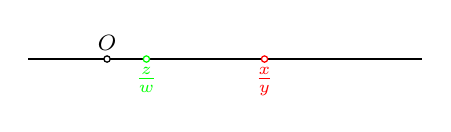
\begin{tikzpicture}
                    % \clip (0,0) rectangle (14.000000,10.000000);
                    {\footnotesize
                    
                    % Drawing segment A B
                    \draw [line width=0.016cm] (1.000000,1.500000) -- (1.960000,1.500000);%
                    \draw [line width=0.016cm] (2.040000,1.500000) -- (2.460000,1.500000);%
                    \draw [line width=0.016cm] (2.540000,1.500000) -- (3.960000,1.500000);%
                    \draw [line width=0.016cm] (4.040000,1.500000) -- (6.000000,1.500000);%
                    
                    % Marking point O by circle
                    \draw [line width=0.016cm] (2.000000,1.500000) circle (0.040000);%
                    \draw (2.000000,1.500000) node [anchor=south] { $O$ };%
                    
                    % Changing color 255 0 0
                    \definecolor{r255g0b0}{rgb}{1.000000,0.000000,0.000000}%
                    \color{r255g0b0}% 
                    
                    % Marking point \frac{x}{y} by circle
                    \draw [line width=0.016cm] (4.000000,1.500000) circle (0.040000);%
                    \draw (4.000000,1.500000) node [anchor=north] { $\frac{x}{y}$ };%
                    
                    % Changing color 0 255 0
                    \definecolor{r0g255b0}{rgb}{0.000000,1.000000,0.000000}%
                    \color{r0g255b0}% 
                    
                    % Marking point \frac{z}{w} by circle
                    \draw [line width=0.016cm] (2.500000,1.500000) circle (0.040000);%
                    \draw (2.500000,1.500000) node [anchor=north] { $\frac{z}{w}$ };%
                    \color{black}
                    }
                \end{tikzpicture}}    
            \end{block}}

            \only<4->{\begin{block}{}
                Slike pozitivnih racionalnih števil ležijo desno, slike negativnih racionalnih števil pa levo od koordinatnega izhodišča. \\
                \only<5->{\centering
                \begin{tikzpicture}
                    
                    % \clip (0,0) rectangle (14.000000,10.000000);
                    {\footnotesize
                    
                    % Drawing segment A B
                    \draw [line width=0.016cm] (1.000000,1.500000) -- (3.460000,1.500000);%
                    \draw [line width=0.016cm] (3.540000,1.500000) -- (6.000000,1.500000);%
                    
                    % Changing color 255 0 0
                    \definecolor{r255g0b0}{rgb}{1.000000,0.000000,0.000000}%
                    \color{r255g0b0}% 
                    
                    % Drawing segment B O
                    \draw [line width=0.016cm] (6.000000,1.500000) -- (3.540000,1.500000);%
                    
                    % Marking point pozitivna_tevila
                    \draw (4.750000,1.500000) node [anchor=north] { $pozitivna~ števila$ };%
                    \draw (4.750000,1.500000) node [anchor=south] { $\mathbb{Q}^+$ };%
                    
                    % Changing color 0 255 0
                    \definecolor{r0g255b0}{rgb}{0.000000,1.000000,0.000000}%
                    \color{r0g255b0}% 
                    
                    % Drawing segment O A
                    \draw [line width=0.016cm] (3.460000,1.500000) -- (1.000000,1.500000);%
                    
                    % Marking point negativna_tevila
                    \draw (2.250000,1.500000) node [anchor=north] { $negativna~ števila$ };%
                    \draw (2.250000,1.500000) node [anchor=south] { $\mathbb{Q}^-$ };%
                    
                    % Changing color 0 0 0
                    \definecolor{r0g0b0}{rgb}{0.000000,0.000000,0.000000}%
                    \color{r0g0b0}% 
                    
                    % Marking point O by circle
                    \draw [line width=0.032cm] (3.500000,1.500000) circle (0.040000);%
                    \draw (3.500000,1.500000) node [anchor=south] { $O$ };%
                    \color{black}
                    }
                \end{tikzpicture}}
            \end{block}}

            \only<6->{\begin{block}{}
                V množici ulomkov velja, da je vsak negativen ulomek manjši od vsakega pozitivnega ulomka.
            \end{block}}

        \end{frame}

        \begin{frame}
            \textbf{\large{Lastnosti relacije urejenosti}}
            
            \only<2->{\begin{alertblock}{Monotonost vsote}
                \only<3->{Če na obeh straneh neenakosti prištejemo isto število, se neenakost ohrani.}
                \only<4->{$$ \dfrac{x}{y}<\dfrac{z}{w} \quad \Rightarrow \quad \dfrac{x}{y}+\dfrac{r}{q}<\dfrac{z}{w}+\dfrac{r}{q} $$}
                % \only<5->{$$ \mathbf{p<q \quad \Rightarrow \quad p+r<q+r} $$}
            \end{alertblock}}

            \only<6->{\begin{alertblock}{Tranzitivnost}
                \only<7->{$$ \dfrac{x}{y}<\dfrac{z}{w} \quad \wedge \quad \dfrac{z}{w}<\dfrac{r}{q} \quad \Rightarrow \quad \dfrac{x}{y}<\dfrac{r}{q} $$}
                % \only<8->{$$ \mathbf{p<q \quad \wedge \quad q<r \quad \Rightarrow \quad p<r} $$}
            \end{alertblock}}

        \end{frame}

        \begin{frame}

            \only<2->{\begin{alertblock}{}
                Pri množenju neenakosti s pozitivnim številom se znak neenakosti ohrani.
                \only<3->{$$ \dfrac{x}{y}<\dfrac{z}{w} \quad \wedge \quad \dfrac{r}{q}>0 \quad \Rightarrow \quad \dfrac{x}{y}\cdot\dfrac{r}{q}<\dfrac{z}{w}\cdot\dfrac{r}{q} $$}
                % \only<4->{$$ \mathbf{p<q \quad \wedge \quad r>0 \quad \Rightarrow \quad p\cdot r<q\cdot r} $$}
            \end{alertblock}}

            \only<5->{\begin{alertblock}{}
                Pri množenju neenakosti s negativnim številom se znak neenakosti obrne.
                \only<6->{$$ \dfrac{x}{y}<\dfrac{z}{w} \quad \wedge \quad \dfrac{r}{q}<0 \quad \Rightarrow \quad \dfrac{x}{y}\cdot\dfrac{r}{q}>\dfrac{z}{w}\cdot\dfrac{r}{q} $$}
                % \only<7->{$$ \mathbf{p<q \quad \wedge \quad r>0 \quad \Rightarrow \quad p\cdot r>q\cdot r} $$}
            \end{alertblock}}

            \only<8->{\begin{block}{}
                Pri prehodu na nasprotno vrednost se neenačaj obrne:
                \only<9->{$$ \dfrac{x}{y}<\dfrac{z}{w} \quad \Rightarrow \quad -\dfrac{x}{y}>-\dfrac{z}{w} $$}
            \end{block}}



        \end{frame}

        \begin{frame}
            
            \only<2->{\begin{alertblock}{}
                Množica racionalnih števil pa je tudi \textbf{delno urejena}, in sicer z relacijo \textit{biti manjši ali enak} ($\leq$) oziroma \textit{biti večji ali enak} ($\geq$). Za ulomka $\dfrac{x}{y}$ in $\dfrac{z}{w}$ ($b,d\in\mathbb{N}$) velja vsaj ena izmed možnosti:
                \begin{enumerate}
                    \item<3-> prvi ulomek je večji ali enak od drugega $\dfrac{x}{y}\geq\dfrac{z}{w}$ natanko tedaj, ko je $ad\geq bc$;
                    \item<4-> drugi ulomek je večji ali enak od prvega $\dfrac{x}{y}\geq\dfrac{z}{w}$ natanko tedaj, ko je $ad\leq bc$;
                \end{enumerate}
            \end{alertblock}}

            \only<5->{\begin{block}{}
                Za (zgornjo) relacijo delne urejenosti veljajo naslednje lastnosti:
                \begin{itemize}
                    \item<6-> $\dfrac{x}{y}\leq\dfrac{x}{y}$ -- \textbf{refleksivnost};
                    \item<7-> $\dfrac{x}{y}\leq\dfrac{z}{w}  \wedge \dfrac{z}{w}\leq\dfrac{x}{y} \Rightarrow \dfrac{x}{y}=\dfrac{z}{w}$ -- \textbf{antisimetričnost} in
                    \item<8-> $\dfrac{x}{y}\leq\dfrac{z}{w}  \wedge \dfrac{z}{w}\leq\dfrac{r}{q} \Rightarrow \dfrac{x}{y}\leq\dfrac{r}{q}$ -- \textbf{tranzitivnost}.
                \end{itemize}
            \end{block}}


        \end{frame}


        \begin{frame}
            \only<2->{\begin{exampleblock}{Naloga}
                Kateri od ulomkov je večji?
                \only<3->{\begin{itemize}
                    \item $\dfrac{3}{7}$, $\dfrac{3}{8}$ \\~\\~
                    \item $\dfrac{7}{3}$, $\dfrac{8}{3}$ \\~\\~
                    \item $\dfrac{2}{5}$, $\dfrac{3}{10}$ \\~\\~
                    \item $\dfrac{1}{100}$, $\dfrac{1}{200}$ \\~\\~
                \end{itemize}}
            \end{exampleblock}}
        \end{frame}

        \begin{frame}
            \only<2->{\begin{exampleblock}{Naloga}
                Katero število je za $\dfrac{3}{5}$ večje od $\dfrac{2}{3}$?
                \\~\\~\\~\\~
            \end{exampleblock}}

            \only<3->{\begin{exampleblock}{Naloga}
                Katero število je za $\dfrac{1}{3}$ manjše od $\dfrac{7}{9}$?
                \\~\\~\\~\\~
            \end{exampleblock}}
        \end{frame}

        \begin{frame}
            \only<2->{\begin{exampleblock}{Naloga}
                Ulomke uredite po velikosti od večjega k manjšemu.
                \only<3->{\begin{itemize}
                    \item $\dfrac{2}{5}$, $\dfrac{3}{10}$, $\dfrac{8}{9}$ in $\dfrac{7}{8}$ \\~\\~\\~\\~
                    \item $-\dfrac{1}{2}$, $\dfrac{-1}{3}$, $\dfrac{-3}{4}$ in $\dfrac{2}{-5}$ \\~\\~\\~\\~
                \end{itemize}}
            \end{exampleblock}}
        \end{frame}


        \begin{frame}
            \only<2->{\begin{exampleblock}{Naloga}
                Ali obstajajo ulomki z imenovalcem $25$, ki so med $\dfrac{4}{9}$ in $\dfrac{5}{9}$? Če obstajajo, jih zapišite.
                \\~\\~\\~\\~
            \end{exampleblock}}

            \only<3->{\begin{exampleblock}{Naloga}
                Ali obstajajo ulomki z imenovalcem $100$, ki so med $\dfrac{13}{53}$ in $\dfrac{14}{53}$? Če obstajajo, jih zapišite.
                \\~\\~\\~\\~
            \end{exampleblock}}
        \end{frame}

        % \begin{frame}
        %     \only<2->{\begin{exampleblock}{Naloga}
        %         Poenostavite.
        %         \only<3->{\begin{itemize}
        %             \item a \\~
        %         \end{itemize}}
        %     \end{exampleblock}}
        % \end{frame}


    \subsection{Potence s celimi eksponenti}

        \begin{frame}
            \frametitle{Potence s celimi eksponenti}
        \end{frame}

        \begin{frame}
            \only<2->{\begin{exampleblock}{Naloga}
                Poenostavite.
                \only<3->{\begin{itemize}
                    \item $x^{10}:x^5$ \\~\\~
                    \item $b^4:b^{-11}$ \\~\\~
                    \item $y^{-3}:y^2$ \\~\\~
                \end{itemize}}
            \end{exampleblock}}
        \end{frame}

        \begin{frame}
            \only<2->{\begin{exampleblock}{Naloga}
                Poenostavite.
                \only<3->{\begin{itemize}
                    \item $\dfrac{x^3y^{-2}}{x^{-2}y^3}$ \\~\\~
                    \item $\dfrac{2^{10}a^4b^{-4}}{2^{-2}a^{-2}b}$ \\~\\~
                    \item $\dfrac{3^{10}x^{-12}y^{-20}}{6^{10}x^2y^{-3}}$ \\~\\~
                \end{itemize}}
            \end{exampleblock}}
        \end{frame}


        \begin{frame}
            \only<2->{\begin{exampleblock}{Naloga}
                Poenostavite.
                \only<3->{\begin{itemize}
                    \item $\left(\dfrac{-2^5a^{-4}b^3}{2^{-2}ab^{-2}}\right)^2:\left(-\dfrac{a^2b^4}{2^3a^{-2}}\right)^3$ \\~\\~
                    \item $\left(\dfrac{-3^4x^{-2}y^3}{x^3z^2}\right)^{-4}\cdot\left(\dfrac{3^5x^2z^{-2}}{y^{-3}}\right)^3$ \\~\\~
                    \item $-\dfrac{5^5a^4b^{-3}}{a^{-3}b^2}:\left(-\dfrac{5^2a^{-2}b}{a^2}\right)^2$ \\~\\~
                \end{itemize}}
            \end{exampleblock}}
        \end{frame}


        \begin{frame}
            \only<2->{\begin{exampleblock}{Naloga}
                Poenostavite.
                \only<3->{\begin{itemize}
                    \item $\dfrac{x^{-2}+x^{-1}}{x^{-3}+x^{-2}}$ \\~\\~
                    \item $\dfrac{x^{-1}+x^{-2}+x^{-3}}{x^{-4}-x^{-1}}$ \\~\\~
                    \item $\dfrac{1+x^{-2}}{x^{-4}-1}$ \\~\\~
                    \item $\dfrac{x^{-2}+x^{-3}}{x^{-3}-x^{-2}}$ \\~\\~
                \end{itemize}}
            \end{exampleblock}}
        \end{frame}


        
        \begin{frame}
            \only<2->{\begin{exampleblock}{Naloga}
                Poenostavite.
                \only<3->{\begin{itemize}
                    \item $\dfrac{3^{n+2}-2\cdot 3^{n-1}}{3^{n-2}+3^n}$ \\~\\~
                    \item $\dfrac{5^{2n}+5^{2n-1}-2\cdot 5^{2n+1}}{25^n}$ \\~\\~
                    \item $\dfrac{7^{3n-3}+3\cdot 7^{3n-2}-7^{3n-4}}{7^{3n-2}-7^{3n-1}}$ \\~\\~
                    \item $\dfrac{2^{n-1}+3\cdot 2^n}{4^n+5\cdot 2^{2n-1}}$ \\~\\~
                \end{itemize}}
            \end{exampleblock}}

        \end{frame}

        \begin{frame}
            \only<2->{\begin{exampleblock}{Naloga}
                Napišite brez negativnih eksponentov.
                \only<3->{\begin{itemize}
                    \item $x^{-1}+2x^{-2}$ \\~
                    \item $1-x^{-1}-x^{-2}$ \\~
                    \item $\dfrac{1}{x^{-1}}+x^{-1}$ \\~\\~
                    \item $\left(\dfrac{\dfrac{2}{x^{-2}}}{\left(x^{-2}\right)^{-1}}\right)^{-1}$ \\~\\~
                \end{itemize}}
            \end{exampleblock}}
        \end{frame}
        

        \begin{frame}
            \only<2->{\begin{exampleblock}{Naloga}
                Poenostavite.
                \only<3->{\begin{itemize}
                    \item $\left(x-x^{-1}\right)\cdot\left(x^2-1\right)^{-1}$ \\~\\~
                    \item $\dfrac{x^{-2}+x^{-1}}{x^{-2}-x^{-1}}-\left(1-x\right)^{-1}$ \\~\\~
                    \item $\left(\dfrac{x^{-3}-x^{-1}}{1-x^{-2}}\right)^{-1}+\left(\dfrac{1}{x}\right)^{-1}$ \\~\\~
                    \item $\left(x^{-2}-2x^{-1}+1\right)^{-1}-\left(x-1\right)^{-2}$ \\~\\~
                \end{itemize}}
            \end{exampleblock}}
        \end{frame}


        % \begin{frame}
        %     \only<2->{\begin{exampleblock}{Naloga}
        %         Poenostavite.
        %         \only<3->{\begin{itemize}
        %             \item a \\~
        %         \end{itemize}}
        %     \end{exampleblock}}
        % \end{frame}


        % \begin{frame}
        %     \only<2->{\begin{exampleblock}{Naloga}
        %         Poenostavite.
        %         \only<3->{\begin{itemize}
        %             \item a \\~
        %         \end{itemize}}
        %     \end{exampleblock}}
        % \end{frame}


        


    \subsection{Decimalni zapis}

        \begin{frame}
            \frametitle{Decimalni zapis}
        \end{frame}

